\documentclass{article}
\usepackage{ctex}
\title{编译原理 作业2}
\author{} 
\date{}
\usepackage[a4paper,left=10mm,right=10mm,top=15mm,bottom=15mm]{geometry} 
\usepackage{graphicx} 
\usepackage{tikz}
\usepackage{makecell}

\begin{document}
\section*{3.7}
\noindent 
\textbf{(1)}首先构造如下图所示的NFA,初态为X,终态为Y:
\begin{center}
    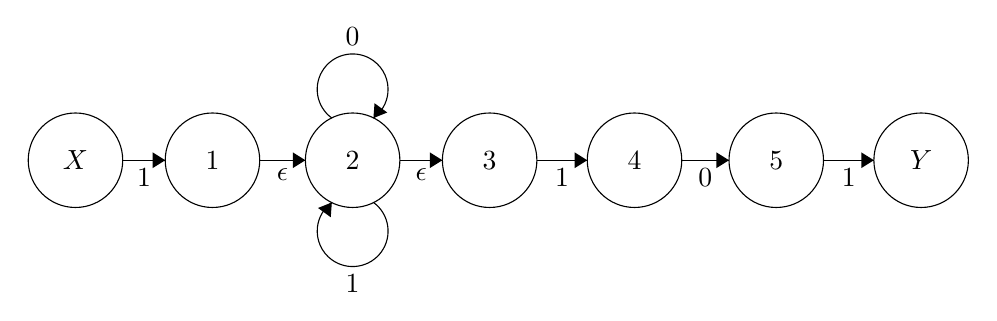
\begin{tikzpicture}[scale=0.2]
    \tikzstyle{every node}+=[inner sep=0pt]
    \draw [black] (5.9,-29.6) circle (3);
    \draw (5.9,-29.6) node {$X$};
    \draw [black] (23.5,-29.6) circle (3);
    \draw (23.5,-29.6) node {$2$};
    \draw [black] (32.2,-29.6) circle (3);
    \draw (32.2,-29.6) node {$3$};
    \draw [black] (14.6,-29.6) circle (3);
    \draw (14.6,-29.6) node {$1$};
    \draw [black] (41.4,-29.6) circle (3);
    \draw (41.4,-29.6) node {$4$};
    \draw [black] (50.4,-29.6) circle (3);
    \draw (50.4,-29.6) node {$5$};
    \draw [black] (59.6,-29.6) circle (3);
    \draw (59.6,-29.6) node {$Y$};
    \draw [black] (8.9,-29.6) -- (11.6,-29.6);
    \fill [black] (11.6,-29.6) -- (10.8,-29.1) -- (10.8,-30.1);
    \draw (10.25,-30.1) node [below] {$1$};
    \draw [black] (17.6,-29.6) -- (20.5,-29.6);
    \fill [black] (20.5,-29.6) -- (19.7,-29.1) -- (19.7,-30.1);
    \draw (19.05,-30.1) node [below] {$\epsilon$};
    \draw [black] (26.5,-29.6) -- (29.2,-29.6);
    \fill [black] (29.2,-29.6) -- (28.4,-29.1) -- (28.4,-30.1);
    \draw (27.85,-30.1) node [below] {$\epsilon$};
    \draw [black] (35.2,-29.6) -- (38.4,-29.6);
    \fill [black] (38.4,-29.6) -- (37.6,-29.1) -- (37.6,-30.1);
    \draw (36.8,-30.1) node [below] {$1$};
    \draw [black] (44.4,-29.6) -- (47.4,-29.6);
    \fill [black] (47.4,-29.6) -- (46.6,-29.1) -- (46.6,-30.1);
    \draw (45.9,-30.1) node [below] {$0$};
    \draw [black] (53.4,-29.6) -- (56.6,-29.6);
    \fill [black] (56.6,-29.6) -- (55.8,-29.1) -- (55.8,-30.1);
    \draw (55,-30.1) node [below] {$1$};
    \draw [black] (22.177,-26.92) arc (234:-54:2.25);
    \draw (23.5,-22.35) node [above] {$0$};
    \fill [black] (24.82,-26.92) -- (25.7,-26.57) -- (24.89,-25.98);
    \draw [black] (24.823,-32.28) arc (54:-234:2.25);
    \draw (23.5,-36.85) node [below] {$1$};
    \fill [black] (22.18,-32.28) -- (21.3,-32.63) -- (22.11,-33.22);
    \end{tikzpicture}
\end{center}
状态转换矩阵为:\\
\begin{table}[h]
    \centering
\begin{tabular}{|p{3cm}<{\centering}|p{3cm}<{\centering}|p{3cm}<{\centering}|}   
    \hline
    $I$ & $I_0$ & $I_1$ \\
    \hline
    $\{X\}$ & $\Phi$ & $\{1,2,3\}$ \\
    \hline
    $\{1,2,3\}$ & $\{2,3\}$ & $\{2,3,4\}$ \\
    \hline
    $\{2,3\}$ & $\{2,3\}$ & $\{2,3,4\}$ \\
    \hline
    $\{2,3,4\}$ & $\{2,3,5\}$ & $\{2,3,4\}$ \\
    \hline
    $\{2,3,5\}$ & $\{2,3\}$ & $\{2,3,4,Y\}$\\
    \hline
    $\{2,3,4,Y\}$ & $\{2,3,5\}$ & $\{2,3,4\}$\\
    \hline
\end{tabular}
\end{table}
\\
对状态子集重命名,可得状态转换矩阵为:
\begin{table}[h]
    \centering
\begin{tabular}{|p{3cm}<{\centering}|p{3cm}<{\centering}|p{3cm}<{\centering}|}   
    \hline
    $s$ & $0$ & $1$ \\
    \hline
    $0$ & $6$ & $1$ \\
    \hline
    $1$ & $2$ & $3$ \\
    \hline
    $2$ & $2$ & $3$ \\
    \hline
    $3$ & $4$ & $3$ \\
    \hline
    $4$ & $2$ & $5$ \\
    \hline
    $5$ & $4$ & $3$ \\
    \hline
\end{tabular}
\end{table}
\\
则初态为0的DFA如下图所示:
\begin{center}
    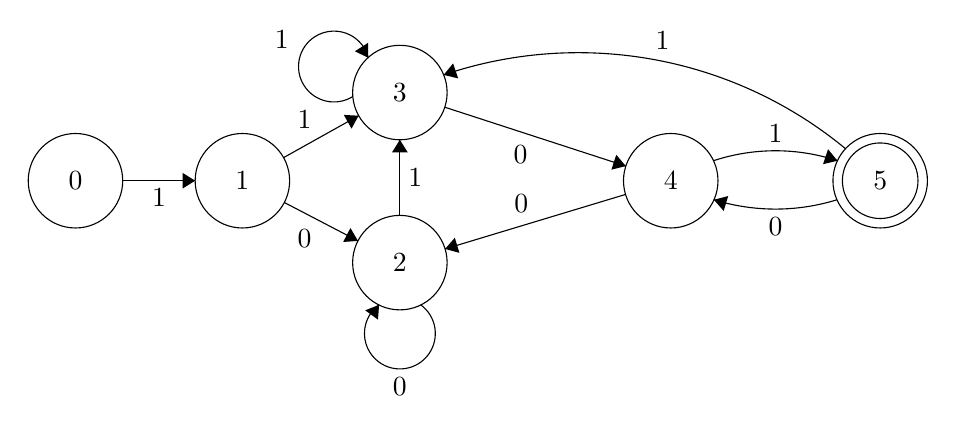
\begin{tikzpicture}[scale=0.2]
    \tikzstyle{every node}+=[inner sep=0pt]
    \draw [black] (11.2,-10.2) circle (3);
    \draw (11.2,-10.2) node {$0$};
    \draw [black] (21.8,-10.2) circle (3);
    \draw (21.8,-10.2) node {$1$};
    \draw [black] (31.8,-15.4) circle (3);
    \draw (31.8,-15.4) node {$2$};
    \draw [black] (31.8,-4.6) circle (3);
    \draw (31.8,-4.6) node {$3$};
    \draw [black] (49,-10.2) circle (3);
    \draw (49,-10.2) node {$4$};
    \draw [black] (62.3,-10.2) circle (3);
    \draw (62.3,-10.2) node {$5$};
    \draw [black] (62.3,-10.2) circle (2.4);
    \draw [black] (14.2,-10.2) -- (18.8,-10.2);
    \fill [black] (18.8,-10.2) -- (18,-9.7) -- (18,-10.7);
    \draw (16.5,-10.7) node [below] {$1$};
    \draw [black] (24.46,-11.58) -- (29.14,-14.02);
    \fill [black] (29.14,-14.02) -- (28.66,-13.2) -- (28.2,-14.09);
    \draw (25.75,-13.3) node [below] {$0$};
    \draw [black] (24.42,-8.73) -- (29.18,-6.07);
    \fill [black] (29.18,-6.07) -- (28.24,-6.02) -- (28.73,-6.89);
    \draw (25.75,-6.9) node [above] {$1$};
    \draw [black] (33.123,-18.08) arc (54:-234:2.25);
    \draw (31.8,-22.65) node [below] {$0$};
    \fill [black] (30.48,-18.08) -- (29.6,-18.43) -- (30.41,-19.02);
    \draw [black] (31.8,-12.4) -- (31.8,-7.6);
    \fill [black] (31.8,-7.6) -- (31.3,-8.4) -- (32.3,-8.4);
    \draw (32.3,-10) node [right] {$1$};
    \draw [black] (28.822,-4.846) arc (302.45713:14.45713:2.25);
    \draw (24.77,-1.25) node [left] {$1$};
    \fill [black] (29.79,-2.39) -- (29.79,-1.44) -- (28.94,-1.98);
    \draw [black] (34.65,-5.53) -- (46.15,-9.27);
    \fill [black] (46.15,-9.27) -- (45.54,-8.55) -- (45.23,-9.5);
    \draw (39.47,-7.94) node [below] {$0$};
    \draw [black] (46.13,-11.07) -- (34.67,-14.53);
    \fill [black] (34.67,-14.53) -- (35.58,-14.78) -- (35.29,-13.82);
    \draw (39.51,-12.25) node [above] {$0$};
    \draw [black] (51.71,-8.93) arc (108.27724:71.72276:12.564);
    \fill [black] (59.59,-8.93) -- (58.99,-8.2) -- (58.67,-9.15);
    \draw (55.65,-7.8) node [above] {$1$};
    \draw [black] (59.561,-11.407) arc (-72.74171:-107.25829:13.181);
    \fill [black] (51.74,-11.41) -- (52.36,-12.12) -- (52.65,-11.17);
    \draw (55.65,-12.5) node [below] {$0$};
    \draw [black] (34.581,-3.479) arc (108.72769:50.4643:26.647);
    \fill [black] (34.58,-3.48) -- (35.5,-3.7) -- (35.18,-2.75);
    \draw (48.48,-1.91) node [above] {$1$};
    \end{tikzpicture}
    \end{center}
\ \\
\textbf{(2)}首先构造初态为0的NFA如下图所示:
\begin{center}
    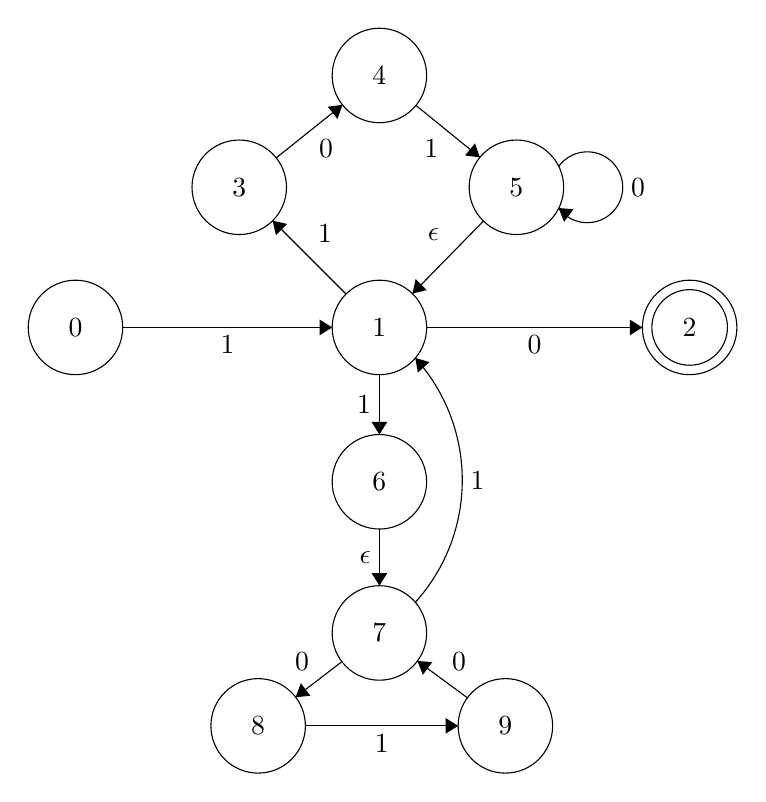
\begin{tikzpicture}[scale=0.2]
    \tikzstyle{every node}+=[inner sep=0pt]
    \draw [black] (20.2,-23.6) circle (3);
    \draw (20.2,-23.6) node {$0$};
    \draw [black] (39.5,-23.6) circle (3);
    \draw (39.5,-23.6) node {$1$};
    \draw [black] (59.2,-23.6) circle (3);
    \draw (59.2,-23.6) node {$2$};
    \draw [black] (59.2,-23.6) circle (2.4);
    \draw [black] (30.6,-14.7) circle (3);
    \draw (30.6,-14.7) node {$3$};
    \draw [black] (39.5,-7.6) circle (3);
    \draw (39.5,-7.6) node {$4$};
    \draw [black] (48.2,-14.7) circle (3);
    \draw (48.2,-14.7) node {$5$};
    \draw [black] (39.5,-33.4) circle (3);
    \draw (39.5,-33.4) node {$6$};
    \draw [black] (39.5,-43) circle (3);
    \draw (39.5,-43) node {$7$};
    \draw [black] (31.8,-48.9) circle (3);
    \draw (31.8,-48.9) node {$8$};
    \draw [black] (47.5,-48.9) circle (3);
    \draw (47.5,-48.9) node {$9$};
    \draw [black] (23.2,-23.6) -- (36.5,-23.6);
    \fill [black] (36.5,-23.6) -- (35.7,-23.1) -- (35.7,-24.1);
    \draw (29.85,-24.1) node [below] {$1$};
    \draw [black] (42.5,-23.6) -- (56.2,-23.6);
    \fill [black] (56.2,-23.6) -- (55.4,-23.1) -- (55.4,-24.1);
    \draw (49.35,-24.1) node [below] {$0$};
    \draw [black] (37.38,-21.48) -- (32.72,-16.82);
    \fill [black] (32.72,-16.82) -- (32.93,-17.74) -- (33.64,-17.03);
    \draw (35.57,-17.67) node [right] {$1$};
    \draw [black] (32.95,-12.83) -- (37.15,-9.47);
    \fill [black] (37.15,-9.47) -- (36.22,-9.58) -- (36.84,-10.36);
    \draw (36.11,-11.64) node [below] {$0$};
    \draw [black] (41.82,-9.5) -- (45.88,-12.8);
    \fill [black] (45.88,-12.8) -- (45.57,-11.91) -- (44.94,-12.68);
    \draw (42.79,-11.64) node [below] {$1$};
    \draw [black] (50.88,-13.377) arc (144:-144:2.25);
    \draw (55.45,-14.7) node [right] {$0$};
    \fill [black] (50.88,-16.02) -- (51.23,-16.9) -- (51.82,-16.09);
    \draw [black] (46.1,-16.85) -- (41.6,-21.45);
    \fill [black] (41.6,-21.45) -- (42.51,-21.23) -- (41.8,-20.53);
    \draw (43.32,-17.68) node [left] {$\epsilon$};
    \draw [black] (39.5,-26.6) -- (39.5,-30.4);
    \fill [black] (39.5,-30.4) -- (40,-29.6) -- (39,-29.6);
    \draw (39,-28.5) node [left] {$1$};
    \draw [black] (39.5,-36.4) -- (39.5,-40);
    \fill [black] (39.5,-40) -- (40,-39.2) -- (39,-39.2);
    \draw (39,-38.2) node [left] {$\epsilon$};
    \draw [black] (34.8,-48.9) -- (44.5,-48.9);
    \fill [black] (44.5,-48.9) -- (43.7,-48.4) -- (43.7,-49.4);
    \draw (39.65,-49.4) node [below] {$1$};
    \draw [black] (37.12,-44.82) -- (34.18,-47.08);
    \fill [black] (34.18,-47.08) -- (35.12,-46.99) -- (34.51,-46.19);
    \draw (34.59,-45.45) node [above] {$0$};
    \draw [black] (45.09,-47.12) -- (41.91,-44.78);
    \fill [black] (41.91,-44.78) -- (42.26,-45.66) -- (42.86,-44.85);
    \draw (44.56,-45.45) node [above] {$0$};
    \draw [black] (41.776,-25.542) arc (42.10601:-42.10601:11.571);
    \fill [black] (41.78,-25.54) -- (41.94,-26.47) -- (42.68,-25.8);
    \draw (45.26,-33.3) node [right] {$1$};
    \end{tikzpicture}
    \end{center}
则状态转换矩阵为:
\begin{table}[h]
    \centering
\begin{tabular}{|p{3cm}<{\centering}|p{3cm}<{\centering}|p{3cm}<{\centering}|}   
    \hline
    $I$ & $I_0$ & $I_1$ \\
    \hline
    $\{0\}$ & $\Phi$ & $\{1\}$ \\
    \hline
    $\{1\}$ & $\{2\}$ & $\{3,6,7\}$ \\
    \hline
    $\{2\}$ & $\Phi$ & $\Phi$ \\
    \hline
    $\{3,6,7\}$ & $\{4,8\}$ & $\Phi$ \\
    \hline
    $\{4,8\}$ & $\Phi$ & $\{1,5,9\}$ \\
    \hline
    $\{1,5,9\}$ & $\{1,2,5,7\}$ & $\{3,6,7\}$ \\
    \hline
    $\{1,2,5,7\}$ & $\{1,2,5,8\}$ & $\{1,3,6,7\}$ \\
    \hline
    $\{1,2,5,8\}$ & $\{1,2,5\}$ & $\{3,6,7,9\}$ \\
    \hline
    $\{1,3,6,7\}$ & $\{2,4,8\}$ & $\{1,3,6,7\}$ \\
    \hline
    $\{1,2,5\}$ & $\{1,2,5\}$ & $\{3,6,7,9\}$ \\
    \hline
    $\{3,6,7,9\}$ & $\{4,7,8\}$ & $\Phi$ \\
    \hline
    $\{2,4,8\}$ & $\Phi$ & $\{1,5,9\}$ \\
    \hline
    $\{4,7,8\}$ & $\{8\}$ & $\{1,5,9\}$ \\
    \hline
    $\{8\}$ & $\Phi$ & $\{9\}$ \\
    \hline
    $\{9\}$ & $\{7\}$ & $\Phi$ \\
    \hline
    $\{7\}$ & $\{8\}$ & $\{1\}$ \\
    \hline
\end{tabular}
\end{table}
\ \\
对状态子集重命名,可得状态转换矩阵为:
\begin{table}[h!]
    \centering
\begin{tabular}{|p{3cm}<{\centering}|p{3cm}<{\centering}|p{3cm}<{\centering}|}   
    \hline
    $s$ & $0$ & $1$ \\
    \hline
    $X$ & $\Phi$ & $0$ \\
    \hline
    $0$ & $1$ & $2$ \\
    \hline
    $1$ & $\Phi$ & $\Phi$ \\
    \hline
    $2$ & $3$ & $\Phi$ \\
    \hline
    $3$ & $\Phi$ & $4$ \\
    \hline
    $4$ & $5$ & $2$ \\
    \hline
    $5$ & $6$ & $7$ \\
    \hline
    $6$ & $8$ & $9$ \\
    \hline
    $7$ & $10$ & $7$ \\
    \hline
    $8$ & $8$ & $9$ \\
    \hline
    $9$ & $11$ & $\Phi$ \\
    \hline
    $10$ & $\Phi$ & $4$ \\
    \hline
    $11$ & $12$ & $4$ \\
    \hline
    $12$ & $\Phi$ & $13$ \\
    \hline
    $13$ & $14$ & $\Phi$ \\
    \hline
    $14$ & $12$ & $0$ \\
    \hline
\end{tabular}
\end{table}
\ \\ \\ \\ \\ \\ \\ \\ \\ \\
因此,得到以X为初态的DFA如下图所示:
\begin{center}
    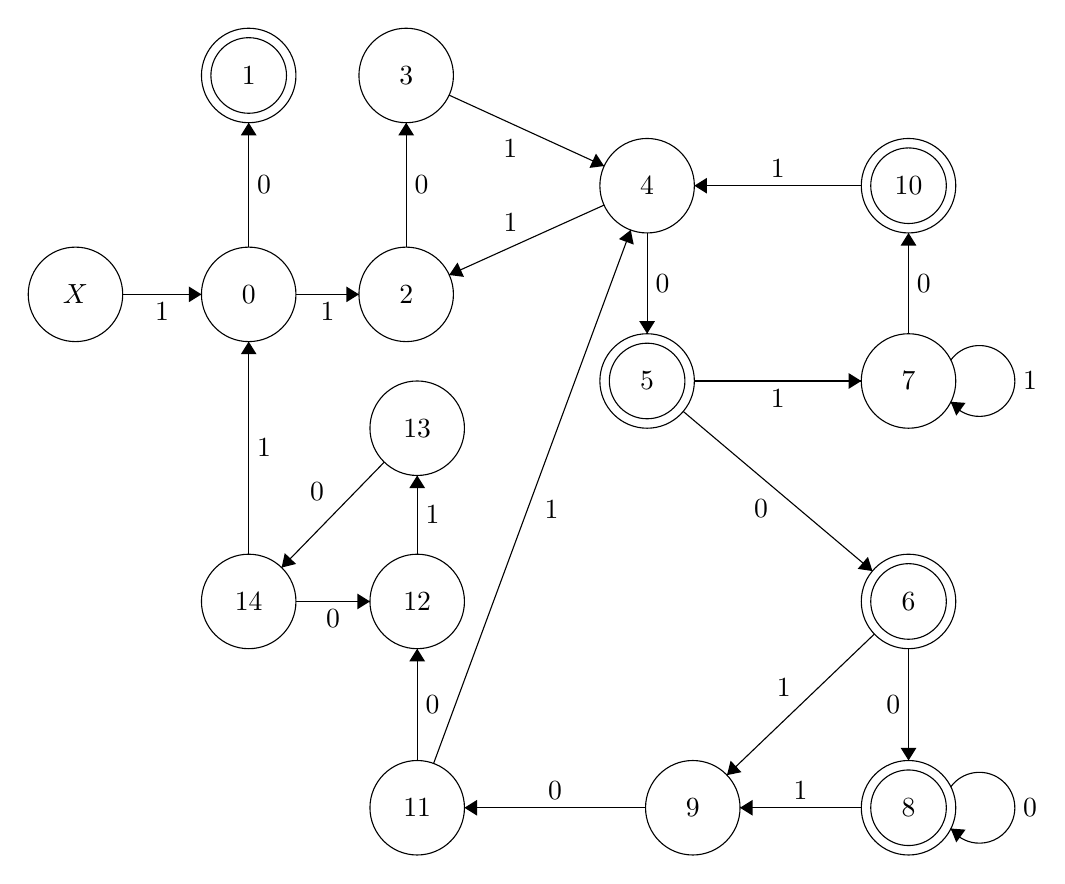
\begin{tikzpicture}[scale=0.2]
    \tikzstyle{every node}+=[inner sep=0pt]
    \draw [black] (6.3,-17.2) circle (3);
    \draw (6.3,-17.2) node {$X$};
    \draw [black] (17.3,-17.2) circle (3);
    \draw (17.3,-17.2) node {$0$};
    \draw [black] (17.3,-3.3) circle (3);
    \draw (17.3,-3.3) node {$1$};
    \draw [black] (17.3,-3.3) circle (2.4);
    \draw [black] (27.3,-17.2) circle (3);
    \draw (27.3,-17.2) node {$2$};
    \draw [black] (27.3,-3.3) circle (3);
    \draw (27.3,-3.3) node {$3$};
    \draw [black] (42.6,-10.3) circle (3);
    \draw (42.6,-10.3) node {$4$};
    \draw [black] (42.6,-22.7) circle (3);
    \draw (42.6,-22.7) node {$5$};
    \draw [black] (42.6,-22.7) circle (2.4);
    \draw [black] (59.2,-36.7) circle (3);
    \draw (59.2,-36.7) node {$6$};
    \draw [black] (59.2,-36.7) circle (2.4);
    \draw [black] (59.2,-22.7) circle (3);
    \draw (59.2,-22.7) node {$7$};
    \draw [black] (59.2,-49.8) circle (3);
    \draw (59.2,-49.8) node {$8$};
    \draw [black] (59.2,-49.8) circle (2.4);
    \draw [black] (45.5,-49.8) circle (3);
    \draw (45.5,-49.8) node {$9$};
    \draw [black] (59.2,-10.3) circle (3);
    \draw (59.2,-10.3) node {$10$};
    \draw [black] (59.2,-10.3) circle (2.4);
    \draw [black] (28,-49.8) circle (3);
    \draw (28,-49.8) node {$11$};
    \draw [black] (28,-36.7) circle (3);
    \draw (28,-36.7) node {$12$};
    \draw [black] (28,-25.7) circle (3);
    \draw (28,-25.7) node {$13$};
    \draw [black] (17.3,-36.7) circle (3);
    \draw (17.3,-36.7) node {$14$};
    \draw [black] (9.3,-17.2) -- (14.3,-17.2);
    \fill [black] (14.3,-17.2) -- (13.5,-16.7) -- (13.5,-17.7);
    \draw (11.8,-17.7) node [below] {$1$};
    \draw [black] (17.3,-14.2) -- (17.3,-6.3);
    \fill [black] (17.3,-6.3) -- (16.8,-7.1) -- (17.8,-7.1);
    \draw (17.8,-10.25) node [right] {$0$};
    \draw [black] (20.3,-17.2) -- (24.3,-17.2);
    \fill [black] (24.3,-17.2) -- (23.5,-16.7) -- (23.5,-17.7);
    \draw (22.3,-17.7) node [below] {$1$};
    \draw [black] (27.3,-14.2) -- (27.3,-6.3);
    \fill [black] (27.3,-6.3) -- (26.8,-7.1) -- (27.8,-7.1);
    \draw (27.8,-10.25) node [right] {$0$};
    \draw [black] (30.03,-4.55) -- (39.87,-9.05);
    \fill [black] (39.87,-9.05) -- (39.35,-8.26) -- (38.94,-9.17);
    \draw (33.91,-7.31) node [below] {$1$};
    \draw [black] (42.6,-13.3) -- (42.6,-19.7);
    \fill [black] (42.6,-19.7) -- (43.1,-18.9) -- (42.1,-18.9);
    \draw (43.1,-16.5) node [right] {$0$};
    \draw [black] (39.87,-11.53) -- (30.03,-15.97);
    \fill [black] (30.03,-15.97) -- (30.97,-16.09) -- (30.56,-15.18);
    \draw (33.92,-13.24) node [above] {$1$};
    \draw [black] (44.89,-24.63) -- (56.91,-34.77);
    \fill [black] (56.91,-34.77) -- (56.62,-33.87) -- (55.97,-34.63);
    \draw (49.84,-30.19) node [below] {$0$};
    \draw [black] (45.6,-22.7) -- (56.2,-22.7);
    \fill [black] (56.2,-22.7) -- (55.4,-22.2) -- (55.4,-23.2);
    \draw (50.9,-23.2) node [below] {$1$};
    \draw [black] (59.2,-39.7) -- (59.2,-46.8);
    \fill [black] (59.2,-46.8) -- (59.7,-46) -- (58.7,-46);
    \draw (58.7,-43.25) node [left] {$0$};
    \draw [black] (57.03,-38.77) -- (47.67,-47.73);
    \fill [black] (47.67,-47.73) -- (48.59,-47.54) -- (47.9,-46.81);
    \draw (51.28,-42.77) node [above] {$1$};
    \draw [black] (59.2,-19.7) -- (59.2,-13.3);
    \fill [black] (59.2,-13.3) -- (58.7,-14.1) -- (59.7,-14.1);
    \draw (59.7,-16.5) node [right] {$0$};
    \draw [black] (61.88,-21.377) arc (144:-144:2.25);
    \draw (66.45,-22.7) node [right] {$1$};
    \fill [black] (61.88,-24.02) -- (62.23,-24.9) -- (62.82,-24.09);
    \draw [black] (61.88,-48.477) arc (144:-144:2.25);
    \draw (66.45,-49.8) node [right] {$0$};
    \fill [black] (61.88,-51.12) -- (62.23,-52) -- (62.82,-51.19);
    \draw [black] (56.2,-49.8) -- (48.5,-49.8);
    \fill [black] (48.5,-49.8) -- (49.3,-50.3) -- (49.3,-49.3);
    \draw (52.35,-49.3) node [above] {$1$};
    \draw [black] (42.5,-49.8) -- (31,-49.8);
    \fill [black] (31,-49.8) -- (31.8,-50.3) -- (31.8,-49.3);
    \draw (36.75,-49.3) node [above] {$0$};
    \draw [black] (56.2,-10.3) -- (45.6,-10.3);
    \fill [black] (45.6,-10.3) -- (46.4,-10.8) -- (46.4,-9.8);
    \draw (50.9,-9.8) node [above] {$1$};
    \draw [black] (28,-46.8) -- (28,-39.7);
    \fill [black] (28,-39.7) -- (27.5,-40.5) -- (28.5,-40.5);
    \draw (28.5,-43.25) node [right] {$0$};
    \draw [black] (29.04,-46.99) -- (41.56,-13.11);
    \fill [black] (41.56,-13.11) -- (40.81,-13.69) -- (41.75,-14.04);
    \draw (36.06,-30.85) node [right] {$1$};
    \draw [black] (28,-33.7) -- (28,-28.7);
    \fill [black] (28,-28.7) -- (27.5,-29.5) -- (28.5,-29.5);
    \draw (28.5,-31.2) node [right] {$1$};
    \draw [black] (25.91,-27.85) -- (19.39,-34.55);
    \fill [black] (19.39,-34.55) -- (20.31,-34.32) -- (19.59,-33.63);
    \draw (22.12,-29.73) node [left] {$0$};
    \draw [black] (20.3,-36.7) -- (25,-36.7);
    \fill [black] (25,-36.7) -- (24.2,-36.2) -- (24.2,-37.2);
    \draw (22.65,-37.2) node [below] {$0$};
    \draw [black] (17.3,-33.7) -- (17.3,-20.2);
    \fill [black] (17.3,-20.2) -- (16.8,-21) -- (17.8,-21);
    \draw (17.8,-26.95) node [right] {$1$};
    \end{tikzpicture}
    \end{center}
\ \\
\textbf{(3)}初态为0的DFA如下图所示:
\begin{center}
    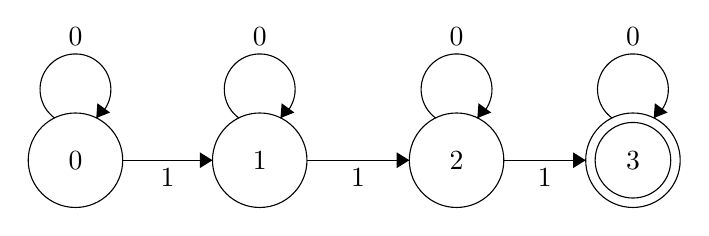
\begin{tikzpicture}[scale=0.2]
    \tikzstyle{every node}+=[inner sep=0pt]
    \draw [black] (8.8,-15.8) circle (3);
    \draw (8.8,-15.8) node {$0$};
    \draw [black] (20.5,-15.8) circle (3);
    \draw (20.5,-15.8) node {$1$};
    \draw [black] (33,-15.8) circle (3);
    \draw (33,-15.8) node {$2$};
    \draw [black] (44.2,-15.8) circle (3);
    \draw (44.2,-15.8) node {$3$};
    \draw [black] (44.2,-15.8) circle (2.4);
    \draw [black] (7.477,-13.12) arc (234:-54:2.25);
    \draw (8.8,-8.55) node [above] {$0$};
    \fill [black] (10.12,-13.12) -- (11,-12.77) -- (10.19,-12.18);
    \draw [black] (19.177,-13.12) arc (234:-54:2.25);
    \draw (20.5,-8.55) node [above] {$0$};
    \fill [black] (21.82,-13.12) -- (22.7,-12.77) -- (21.89,-12.18);
    \draw [black] (23.5,-15.8) -- (30,-15.8);
    \fill [black] (30,-15.8) -- (29.2,-15.3) -- (29.2,-16.3);
    \draw (26.75,-16.3) node [below] {$1$};
    \draw [black] (11.8,-15.8) -- (17.5,-15.8);
    \fill [black] (17.5,-15.8) -- (16.7,-15.3) -- (16.7,-16.3);
    \draw (14.65,-16.3) node [below] {$1$};
    \draw [black] (31.677,-13.12) arc (234:-54:2.25);
    \draw (33,-8.55) node [above] {$0$};
    \fill [black] (34.32,-13.12) -- (35.2,-12.77) -- (34.39,-12.18);
    \draw [black] (36,-15.8) -- (41.2,-15.8);
    \fill [black] (41.2,-15.8) -- (40.4,-15.3) -- (40.4,-16.3);
    \draw (38.6,-16.3) node [below] {$1$};
    \draw [black] (42.877,-13.12) arc (234:-54:2.25);
    \draw (44.2,-8.55) node [above] {$0$};
    \fill [black] (45.52,-13.12) -- (46.4,-12.77) -- (45.59,-12.18);
    \end{tikzpicture}
    \end{center}
\ \\
\textbf{(4)}首先构造NFA,结果如下图所示:
\begin{center}
    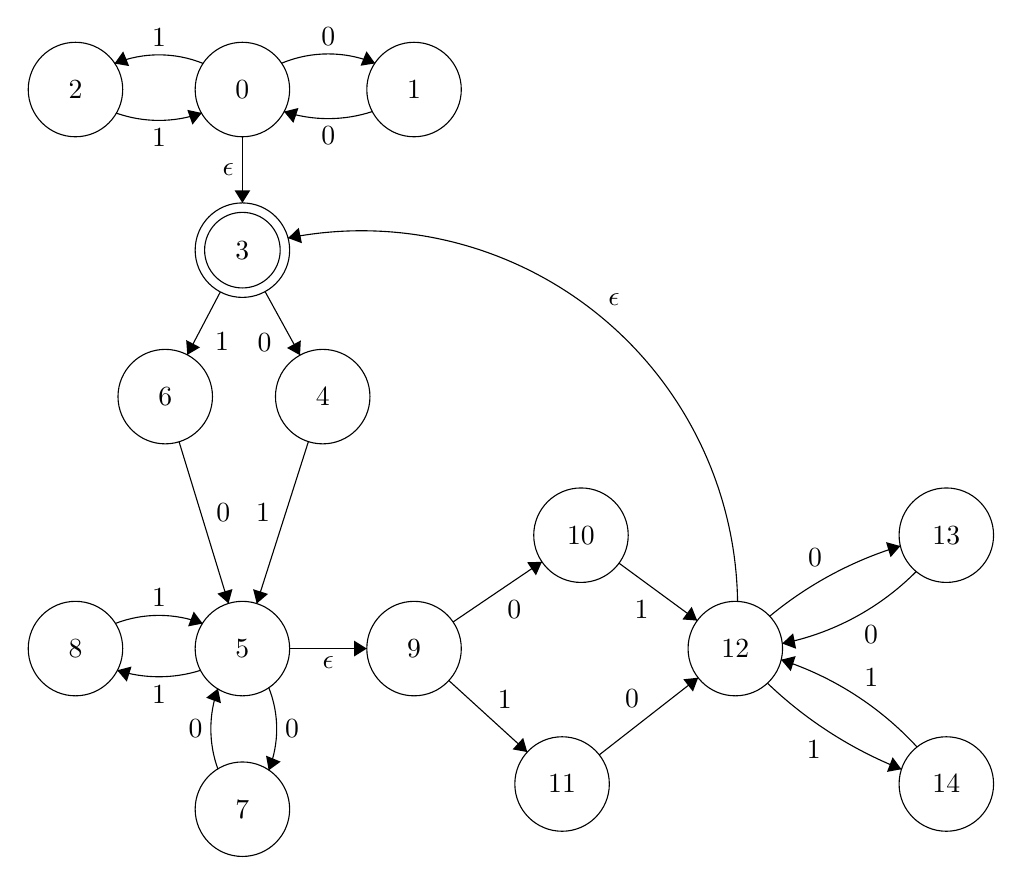
\begin{tikzpicture}[scale=0.2]
    \tikzstyle{every node}+=[inner sep=0pt]
    \draw [black] (14.5,-8.3) circle (3);
    \draw (14.5,-8.3) node {$0$};
    \draw [black] (25.4,-8.3) circle (3);
    \draw (25.4,-8.3) node {$1$};
    \draw [black] (3.9,-8.3) circle (3);
    \draw (3.9,-8.3) node {$2$};
    \draw [black] (14.5,-18.5) circle (3);
    \draw (14.5,-18.5) node {$3$};
    \draw [black] (14.5,-18.5) circle (2.4);
    \draw [black] (19.6,-27.8) circle (3);
    \draw (19.6,-27.8) node {$4$};
    \draw [black] (9.6,-27.8) circle (3);
    \draw (9.6,-27.8) node {$6$};
    \draw [black] (14.5,-43.8) circle (3);
    \draw (14.5,-43.8) node {$5$};
    \draw [black] (14.5,-54) circle (3);
    \draw (14.5,-54) node {$7$};
    \draw [black] (3.9,-43.8) circle (3);
    \draw (3.9,-43.8) node {$8$};
    \draw [black] (25.4,-43.8) circle (3);
    \draw (25.4,-43.8) node {$9$};
    \draw [black] (36,-36.6) circle (3);
    \draw (36,-36.6) node {$10$};
    \draw [black] (34.8,-52.4) circle (3);
    \draw (34.8,-52.4) node {$11$};
    \draw [black] (45.8,-43.8) circle (3);
    \draw (45.8,-43.8) node {$12$};
    \draw [black] (59.2,-36.6) circle (3);
    \draw (59.2,-36.6) node {$13$};
    \draw [black] (59.2,-52.4) circle (3);
    \draw (59.2,-52.4) node {$14$};
    \draw [black] (16.974,-6.637) arc (112.75094:67.24906:7.696);
    \fill [black] (22.93,-6.64) -- (22.38,-5.87) -- (22,-6.79);
    \draw (19.95,-5.54) node [above] {$0$};
    \draw [black] (22.76,-9.696) arc (-71.71955:-108.28045:8.96);
    \fill [black] (17.14,-9.7) -- (17.74,-10.42) -- (18.06,-9.47);
    \draw (19.95,-10.65) node [below] {$0$};
    \draw [black] (6.381,-6.649) arc (112.14872:67.85128:7.478);
    \fill [black] (6.38,-6.65) -- (7.31,-6.81) -- (6.93,-5.88);
    \draw (9.2,-5.6) node [above] {$1$};
    \draw [black] (14.5,-11.3) -- (14.5,-15.5);
    \fill [black] (14.5,-15.5) -- (15,-14.7) -- (14,-14.7);
    \draw (14,-13.4) node [left] {$\epsilon$};
    \draw [black] (15.94,-21.13) -- (18.16,-25.17);
    \fill [black] (18.16,-25.17) -- (18.21,-24.23) -- (17.33,-24.71);
    \draw (16.38,-24.34) node [left] {$0$};
    \draw [black] (13.1,-21.15) -- (11,-25.15);
    \fill [black] (11,-25.15) -- (11.81,-24.67) -- (10.93,-24.21);
    \draw (12.73,-24.31) node [right] {$1$};
    \draw [black] (16.168,-46.267) arc (21.89457:-21.89457:7.062);
    \fill [black] (16.17,-51.53) -- (16.93,-50.98) -- (16,-50.6);
    \draw (17.18,-48.9) node [right] {$0$};
    \draw [black] (12.946,-51.457) arc (-160.04686:-199.95314:7.493);
    \fill [black] (12.95,-46.34) -- (12.2,-46.92) -- (13.14,-47.27);
    \draw (12,-48.9) node [left] {$0$};
    \draw [black] (11.852,-45.178) arc (-72.34227:-107.65773:8.742);
    \fill [black] (6.55,-45.18) -- (7.16,-45.9) -- (7.46,-44.94);
    \draw (9.2,-46.09) node [below] {$1$};
    \draw [black] (6.421,-42.209) arc (111.11028:68.88972:7.715);
    \fill [black] (11.98,-42.21) -- (11.41,-41.45) -- (11.05,-42.39);
    \draw (9.2,-41.19) node [above] {$1$};
    \draw [black] (17.5,-43.8) -- (22.4,-43.8);
    \fill [black] (22.4,-43.8) -- (21.6,-43.3) -- (21.6,-44.3);
    \draw (19.95,-44.3) node [below] {$\epsilon$};
    \draw [black] (27.88,-42.11) -- (33.52,-38.29);
    \fill [black] (33.52,-38.29) -- (32.58,-38.32) -- (33.14,-39.15);
    \draw (31.76,-40.7) node [below] {$0$};
    \draw [black] (27.61,-45.83) -- (32.59,-50.37);
    \fill [black] (32.59,-50.37) -- (32.33,-49.47) -- (31.66,-50.2);
    \draw (31.17,-47.61) node [above] {$1$};
    \draw [black] (47.984,-41.746) arc (129.64288:106.85659:23.843);
    \fill [black] (56.28,-37.29) -- (55.37,-37.04) -- (55.66,-38);
    \draw (50.86,-38.6) node [above] {$0$};
    \draw [black] (56.353,-51.459) arc (-111.57602:-133.80794:26.229);
    \fill [black] (56.35,-51.46) -- (55.79,-50.7) -- (55.43,-51.63);
    \draw (50.78,-49.64) node [below] {$1$};
    \draw [black] (57.289,-38.907) arc (-44.81443:-78.6861:16.582);
    \fill [black] (48.78,-43.48) -- (49.66,-43.81) -- (49.47,-42.83);
    \draw (54.42,-42.33) node [below] {$0$};
    \draw [black] (48.712,-44.511) arc (72.01669:42.59934:20.191);
    \fill [black] (48.71,-44.51) -- (49.32,-45.23) -- (49.63,-44.28);
    \draw (54.44,-46.22) node [above] {$1$};
    \draw [black] (17.397,-17.73) arc (101.28694:0.81537:23.877);
    \fill [black] (17.4,-17.73) -- (18.28,-18.06) -- (18.08,-17.08);
    \draw (38.09,-22.08) node [above] {$\epsilon$};
    \draw [black] (11.918,-9.794) arc (-70.49344:-109.50656:8.141);
    \fill [black] (11.92,-9.79) -- (11,-9.59) -- (11.33,-10.53);
    \draw (9.2,-10.76) node [below] {$1$};
    \draw [black] (10.48,-30.67) -- (13.62,-40.93);
    \fill [black] (13.62,-40.93) -- (13.87,-40.02) -- (12.91,-40.31);
    \draw (12.82,-35.18) node [right] {$0$};
    \draw [black] (18.69,-30.66) -- (15.41,-40.94);
    \fill [black] (15.41,-40.94) -- (16.13,-40.33) -- (15.18,-40.03);
    \draw (16.28,-35.14) node [left] {$1$};
    \draw [black] (38.42,-38.38) -- (43.38,-42.02);
    \fill [black] (43.38,-42.02) -- (43.03,-41.15) -- (42.44,-41.95);
    \draw (39.84,-40.7) node [below] {$1$};
    \draw [black] (37.16,-50.55) -- (43.44,-45.65);
    \fill [black] (43.44,-45.65) -- (42.5,-45.75) -- (43.11,-46.53);
    \draw (39.24,-47.6) node [above] {$0$};
    \end{tikzpicture}
    \end{center}
则状态转换矩阵为:
\begin{table}[h]
    \centering
\begin{tabular}{|p{3cm}<{\centering}|p{3cm}<{\centering}|p{3cm}<{\centering}|}   
    \hline
    $I$ & $I_0$ & $I_1$ \\
    \hline
    $\{0,3\}$ & $\{1,4\}$ & $\{2,6\}$ \\
    \hline
    $\{1,4\}$ & $\{0,3\}$ & $\{5,9\}$ \\
    \hline
    $\{2,6\}$ & $\{5,9\}$ & $\{0,3\}$ \\
    \hline
    $\{5,9\}$ & $\{7,10\}$ & $\{8,11\}$ \\
    \hline
    $\{7,10\}$ & $\{5,9\}$ & $\{12,3\}$ \\
    \hline
    $\{8,11\}$ & $\{12,3\}$ & $\{5,9\}$ \\
    \hline
    $\{12,3\}$ & $\{4,13\}$ & $\{6,14\}$ \\
    \hline
    $\{4,13\}$ & $\{12,3\}$ & $\{5,9\}$ \\
    \hline
    $\{6,14\}$ & $\{5,9\}$ & $\{12,3\}$ \\
    \hline
\end{tabular}
\end{table}
\ \\
对状态子集重命名,可得状态转换矩阵为:
\begin{table}[h]
    \centering

\begin{tabular}{|p{3cm}<{\centering}|p{3cm}<{\centering}|p{3cm}<{\centering}|}   
    \hline
    $s$ & $0$ & $1$ \\
    \hline
    $0$ & $1$ & $2$ \\
    \hline
    $1$ & $0$ & $3$ \\
    \hline
    $2$ & $3$ & $0$ \\
    \hline
    $3$ & $4$ & $5$ \\
    \hline
    $4$ & $3$ & $6$ \\
    \hline
    $5$ & $6$ & $3$ \\
    \hline
    $6$ & $7$ & $8$ \\
    \hline
    $7$ & $6$ & $3$ \\
    \hline
    $8$ & $3$ & $6$ \\
    \hline
\end{tabular}
\end{table}
\ \\
因此,得到以0为初态的DFA如下图所示:
\begin{center}
    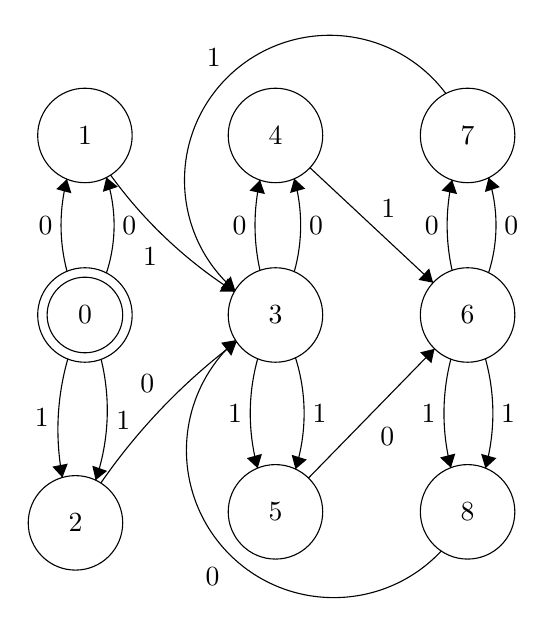
\begin{tikzpicture}[scale=0.2]
    \tikzstyle{every node}+=[inner sep=0pt]
    \draw [black] (8.6,-26) circle (3);
    \draw (8.6,-26) node {$0$};
    \draw [black] (8.6,-26) circle (2.4);
    \draw [black] (8.6,-14.6) circle (3);
    \draw (8.6,-14.6) node {$1$};
    \draw [black] (8,-39.2) circle (3);
    \draw (8,-39.2) node {$2$};
    \draw [black] (20.7,-26) circle (3);
    \draw (20.7,-26) node {$3$};
    \draw [black] (20.7,-14.6) circle (3);
    \draw (20.7,-14.6) node {$4$};
    \draw [black] (20.7,-38.5) circle (3);
    \draw (20.7,-38.5) node {$5$};
    \draw [black] (32.9,-26) circle (3);
    \draw (32.9,-26) node {$6$};
    \draw [black] (32.9,-14.6) circle (3);
    \draw (32.9,-14.6) node {$7$};
    \draw [black] (32.9,-38.5) circle (3);
    \draw (32.9,-38.5) node {$8$};
    \draw [black] (9.963,-17.259) arc (18.27906:-18.27906:9.696);
    \fill [black] (9.96,-17.26) -- (9.74,-18.18) -- (10.69,-17.86);
    \draw (10.95,-20.3) node [right] {$0$};
    \draw [black] (7.464,-23.233) arc (-165.17786:-194.82214:11.464);
    \fill [black] (7.46,-17.37) -- (6.78,-18.01) -- (7.74,-18.27);
    \draw (6.58,-20.3) node [left] {$0$};
    \draw [black] (7.172,-36.321) arc (-169.22646:-195.97866:16.289);
    \fill [black] (7.17,-36.32) -- (7.51,-35.44) -- (6.53,-35.63);
    \draw (6.33,-32.52) node [left] {$1$};
    \draw [black] (9.628,-28.812) arc (13.77973:-18.98485:13.631);
    \fill [black] (9.28,-36.49) -- (10.01,-35.9) -- (9.07,-35.57);
    \draw (10.57,-32.7) node [right] {$1$};
    \draw [black] (18.091,-24.522) arc (-122.50377:-144.08388:28.843);
    \fill [black] (18.09,-24.52) -- (17.68,-23.67) -- (17.15,-24.51);
    \draw (12.74,-21.67) node [below] {$1$};
    \draw [black] (9.61,-36.67) arc (145.31861:126.8933:38.844);
    \fill [black] (18.23,-27.71) -- (17.29,-27.79) -- (17.89,-28.59);
    \draw (13.03,-30.37) node [left] {$0$};
    \draw [black] (19.718,-23.172) arc (-167.3797:-192.6203:13.146);
    \fill [black] (19.72,-17.43) -- (19.05,-18.1) -- (20.03,-18.32);
    \draw (18.9,-20.3) node [left] {$0$};
    \draw [black] (21.893,-17.342) arc (15.67108:-15.67108:10.95);
    \fill [black] (21.89,-17.34) -- (21.63,-18.25) -- (22.59,-17.98);
    \draw (22.8,-20.3) node [right] {$0$};
    \draw [black] (19.572,-35.727) arc (-164.47784:-195.52216:12.994);
    \fill [black] (19.57,-35.73) -- (19.84,-34.82) -- (18.88,-35.09);
    \draw (18.6,-32.25) node [left] {$1$};
    \draw [black] (21.968,-28.71) arc (17.69186:-17.69186:11.649);
    \fill [black] (21.97,-35.79) -- (22.69,-35.18) -- (21.73,-34.88);
    \draw (23.02,-32.25) node [right] {$1$};
    \draw [black] (22.89,-16.65) -- (30.71,-23.95);
    \fill [black] (30.71,-23.95) -- (30.46,-23.04) -- (29.78,-23.77);
    \draw (27.87,-19.82) node [above] {$1$};
    \draw [black] (22.8,-36.35) -- (30.8,-28.15);
    \fill [black] (30.8,-28.15) -- (29.89,-28.37) -- (30.6,-29.07);
    \draw (27.33,-33.72) node [right] {$0$};
    \draw [black] (31.918,-23.172) arc (-167.3797:-192.6203:13.146);
    \fill [black] (31.92,-17.43) -- (31.25,-18.1) -- (32.23,-18.32);
    \draw (31.1,-20.3) node [left] {$0$};
    \draw [black] (34.231,-17.276) arc (17.7798:-17.7798:9.905);
    \fill [black] (34.23,-17.28) -- (34,-18.19) -- (34.95,-17.88);
    \draw (35.2,-20.3) node [right] {$0$};
    \draw [black] (31.839,-35.7) arc (-165.48241:-194.51759:13.764);
    \fill [black] (31.84,-35.7) -- (32.12,-34.8) -- (31.15,-35.05);
    \draw (30.9,-32.25) node [left] {$1$};
    \draw [black] (34.03,-28.772) arc (15.55077:-15.55077:12.973);
    \fill [black] (34.03,-35.73) -- (34.73,-35.09) -- (33.76,-34.82);
    \draw (35,-32.25) node [right] {$1$};
    \draw [black] (18.146,-24.451) arc (-130.56057:-323.3224:9.214);
    \fill [black] (18.15,-24.45) -- (17.86,-23.55) -- (17.21,-24.31);
    \draw (16.78,-10.23) node [above] {$1$};
    \draw [black] (31.235,-40.98) arc (-43.06258:-228.32916:9.355);
    \fill [black] (18.18,-27.6) -- (17.25,-27.76) -- (17.92,-28.51);
    \draw (17.18,-42.6) node [left] {$0$};
    \end{tikzpicture}
    \end{center}
\ \\
\section*{3.8}
\noindent 
\textbf{(1)}$(1|0)*01$\\
\textbf{(2)}$(1|2|3|4|5|6|7|8|9)(0|1|2|3|4|5|6|7|8|9)*(0|5)|(0|5)$\\
\textbf{(3)}$0*1(0|10*1)*|1*0(0|10*1)*$\\
\textbf{(4)}$(A|a)*(B|b)*(C|c)*\dots (Z|z)*$\\
\textbf{(5)}令$d_i = i|\epsilon (i=0,1,\dots,9)$,令$P$表示$0,1,\dots,9$的全排列:\\
$\mathop{\mid}_{i_0i_1\dots i_9\in P}(r_{i_0}r_{i_1}\dots r_{i_9})$\\
\textbf{(6)}
$[\mathop{\mid}_{i\in\{0,1,\dots ,9\}}(r_i)]\cdot [\mathop{\mid}_{i_0i_1\dots i_9\in P}(r_{i_0}r_{i_1}\dots r_{i_9})]$\\
\textbf{(7)}$b*(ab|a)*$
\section*{3.12}
\noindent 
\textbf{(a)}状态转换矩阵为:\\
\begin{table}[h]
    \centering
\begin{tabular}{|p{3cm}<{\centering}|p{3cm}<{\centering}|p{3cm}<{\centering}|}   
    \hline
    $I$ & $I_a$ & $I_b$ \\
    \hline
    $\{0\}$ & $\{0,1\}$ & $\{1\}$ \\
    \hline
    $\{0,1\}$ & $\{0,1\}$ & $\{1\}$ \\
    \hline
    $\{1\}$ & $\{0\}$ & $\Phi$ \\
    \hline
\end{tabular}
\end{table}
\\
对状态子集重命名,可得状态转换矩阵为:
\begin{table}[h]
    \centering
    \begin{tabular}{|p{3cm}<{\centering}|p{3cm}<{\centering}|p{3cm}<{\centering}|}     
        \hline
        s & a & b \\
        \hline
        0 & 1 & 2 \\
        \hline
        1 & 1 & 2 \\
        \hline
        2 & 0 & 3 \\
        \hline
    \end{tabular}
    \end{table}
\\
因此,确定化后以0为初态的有限自动机如下图所示:
\begin{center}
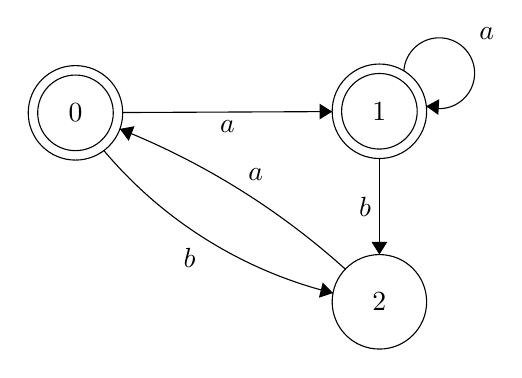
\begin{tikzpicture}[scale=0.2]
\tikzstyle{every node}+=[inner sep=0pt]
\draw [black] (20.3,-19.1) circle (3);
\draw (20.3,-19.1) node {$0$};
\draw [black] (20.3,-19.1) circle (2.4);
\draw [black] (39.6,-19) circle (3);
\draw (39.6,-19) node {$1$};
\draw [black] (39.6,-19) circle (2.4);
\draw [black] (39.6,-31.1) circle (3);
\draw (39.6,-31.1) node {$2$};
\draw [black] (23.3,-19.08) -- (36.6,-19.02);
\fill [black] (36.6,-19.02) -- (35.8,-18.52) -- (35.8,-19.52);
\draw (29.95,-19.56) node [below] {$a$};
\draw [black] (36.654,-30.543) arc (-103.81843:-139.9251:27.644);
\fill [black] (36.65,-30.54) -- (36,-29.87) -- (35.76,-30.84);
\draw (27.54,-27.68) node [below] {$b$};
\draw [black] (41.151,-16.446) arc (176.47119:-111.52881:2.25);
\draw (45.92,-14.07) node [right] {$a$};
\fill [black] (42.57,-18.68) -- (43.34,-19.23) -- (43.4,-18.23);
\draw [black] (39.6,-22) -- (39.6,-28.1);
\fill [black] (39.6,-28.1) -- (40.1,-27.3) -- (39.1,-27.3);
\draw (39.1,-25.05) node [left] {$b$};
\draw [black] (23.12,-20.123) arc (68.26642:47.99005:47.883);
\fill [black] (23.12,-20.12) -- (23.68,-20.88) -- (24.05,-19.95);
\draw (31.74,-23.44) node [above] {$a$};
\end{tikzpicture}
\end{center}
\ \\
将状态划分为终态组$\{0,1\}$和非终态组$\{2\}$,$\{0,1\}_a=\{1\},\{0,1\}_b=\{2\}$,故$\{0,1\}$不可划分.\\
$\{2\}_a=\{0\}$,因此每个组不可再分,则最小化后的以0为初态的自动机如下图所示:
\begin{center}
    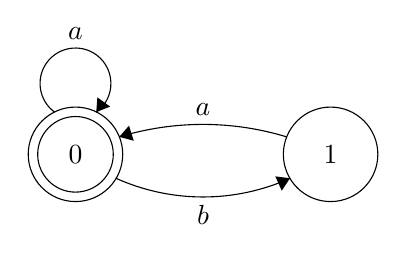
\begin{tikzpicture}[scale=0.2]
    \tikzstyle{every node}+=[inner sep=0pt]
    \draw [black] (32.8,-30.4) circle (3);
    \draw (32.8,-30.4) node {$0$};
    \draw [black] (32.8,-30.4) circle (2.4);
    \draw [black] (49,-30.4) circle (3);
    \draw (49,-30.4) node {$1$};
    \draw [black] (31.477,-27.72) arc (234:-54:2.25);
    \draw (32.8,-23.15) node [above] {$a$};
    \fill [black] (34.12,-27.72) -- (35,-27.37) -- (34.19,-26.78);
    \draw [black] (46.423,-31.924) arc (-65.77928:-114.22072:13.463);
    \fill [black] (46.42,-31.92) -- (45.49,-31.8) -- (45.9,-32.71);
    \draw (40.9,-33.61) node [below] {$b$};
    \draw [black] (35.584,-29.293) arc (106.96846:73.03154:18.213);
    \fill [black] (35.58,-29.29) -- (36.5,-29.54) -- (36.2,-28.58);
    \draw (40.9,-28) node [above] {$a$};
    \end{tikzpicture}
\end{center}
\ \\
\textbf{(b)}
该自动机已经确定化,现在需要进行最小化.首先划分为终态组$\{0,1\}$和非终态组$\{2,3,4,5\}$.\\
显然$\{0,1\}$不可划分,考虑$\{2,3,4,5\}$,由于$\{2,3,4,5\}_a=\{0,1,3,5\}$,这一子集需要划分.\\
考虑到状态2和4通向不同的子集,可将$\{2,3,4,5\}$划分为$\{2,4\},\{3,5\}$.\\
划分后可以发现每个组都不能再分,则以0为初态的DFA如下图所示:
\begin{center}
    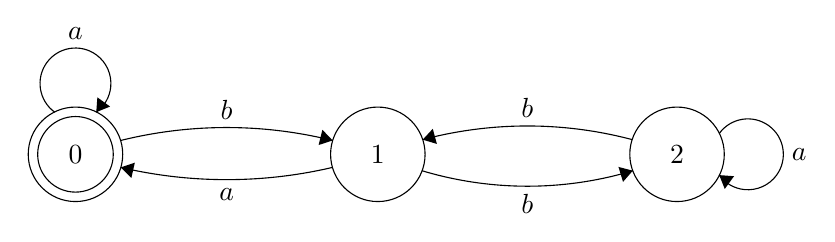
\begin{tikzpicture}[scale=0.2]
    \tikzstyle{every node}+=[inner sep=0pt]
    \draw [black] (14.7,-13) circle (3);
    \draw (14.7,-13) node {$0$};
    \draw [black] (14.7,-13) circle (2.4);
    \draw [black] (33.9,-13) circle (3);
    \draw (33.9,-13) node {$1$};
    \draw [black] (52.9,-13) circle (3);
    \draw (52.9,-13) node {$2$};
    \draw [black] (13.377,-10.32) arc (234:-54:2.25);
    \draw (14.7,-5.75) node [above] {$a$};
    \fill [black] (16.02,-10.32) -- (16.9,-9.97) -- (16.09,-9.38);
    \draw [black] (17.567,-12.122) arc (103.94138:76.05862:27.945);
    \fill [black] (31.03,-12.12) -- (30.38,-11.44) -- (30.14,-12.41);
    \draw (24.3,-10.8) node [above] {$b$};
    \draw [black] (31.019,-13.832) arc (-76.81431:-103.18569:29.455);
    \fill [black] (17.58,-13.83) -- (18.25,-14.5) -- (18.47,-13.53);
    \draw (24.3,-15.11) node [below] {$a$};
    \draw [black] (50.09,-14.044) arc (-73.30567:-106.69433:23.288);
    \fill [black] (50.09,-14.04) -- (49.18,-13.8) -- (49.47,-14.75);
    \draw (43.4,-15.53) node [below] {$b$};
    \draw [black] (55.58,-11.677) arc (144:-144:2.25);
    \draw (60.15,-13) node [right] {$a$};
    \fill [black] (55.58,-14.32) -- (55.93,-15.2) -- (56.52,-14.39);
    \draw [black] (36.749,-12.066) arc (104.83889:75.16111:25.969);
    \fill [black] (36.75,-12.07) -- (37.65,-12.34) -- (37.39,-11.38);
    \draw (43.4,-10.7) node [above] {$b$};
    \end{tikzpicture}
\end{center}

\section*{3.14}
\noindent 

初态为0的DFA如下图所示:\\
\begin{center}
    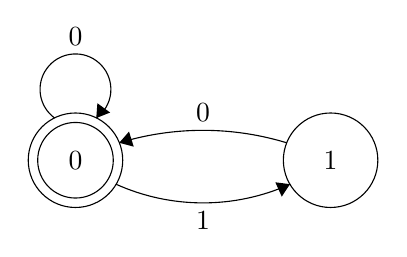
\begin{tikzpicture}[scale=0.2]
    \tikzstyle{every node}+=[inner sep=0pt]
    \draw [black] (32.8,-30.4) circle (3);
    \draw (32.8,-30.4) node {$0$};
    \draw [black] (32.8,-30.4) circle (2.4);
    \draw [black] (49,-30.4) circle (3);
    \draw (49,-30.4) node {$1$};
    \draw [black] (31.477,-27.72) arc (234:-54:2.25);
    \draw (32.8,-23.15) node [above] {$0$};
    \fill [black] (34.12,-27.72) -- (35,-27.37) -- (34.19,-26.78);
    \draw [black] (46.423,-31.924) arc (-65.77928:-114.22072:13.463);
    \fill [black] (46.42,-31.92) -- (45.49,-31.8) -- (45.9,-32.71);
    \draw (40.9,-33.61) node [below] {$1$};
    \draw [black] (35.584,-29.293) arc (106.96846:73.03154:18.213);
    \fill [black] (35.58,-29.29) -- (36.5,-29.54) -- (36.2,-28.58);
    \draw (40.9,-28) node [above] {$0$};
    \end{tikzpicture}
\end{center}
\end{document}
